\documentclass[titlepage]{article}   	% use "amsart" instead of "article" for AMSLaTeX format
\usepackage{geometry}                		% See geometry.pdf to learn the layout options. There are lots.
\geometry{letterpaper}                   		% ... or a4paper or a5paper or ... 
%\geometry{landscape}                		% Activate for rotated page geometry
%\usepackage[parfill]{parskip}    		% Activate to begin paragraphs with an empty line rather than an indent
\usepackage{graphicx}				% Use pdf, png, jpg, or eps§ with pdflatex; use eps in DVI mode
								% TeX will automatically convert eps --> pdf in pdflatex		
\usepackage{amssymb}
\usepackage{dcolumn}
\usepackage[capposition=top]{floatrow}
\usepackage{booktabs}
\usepackage{rotating,tabularx}

%SetFonts
%[11pt, oneside]
%SetFonts


\title{Exploring the Correlates of Homelessness in Los Angeles: A Generalized Additive Approach}
\author{David K. Kirui}
\date{March 1, 2017}							% Activate to display a given date or no date

\begin{document}
\maketitle{}
\section{Introduction: Statement of the Problem}
%\subsection{}

\setlength{\parindent}{10ex} 
Homelessness has been and remains a pressing public policy concern nationwide, as municipalities large and small devise ways of addressing the root causes of homelessness to help alleviate its impact. A key aspect of any public policy aimed at addressing urban homelessness is the collection and maintenance of reliable data on the homeless population. Homelessness is of particular concern to the city and county of Los Angeles, California. Los Angeles, a city of about four million residents and county of about 10 million, has in recent years cultivated the dubious distinction of having the largest number of chronically homeless people in the country. Politicians and policy makers in Los Angeles must have reliable data on the location and prevalence of homelessness in their city and county in order to make meaningful and effective policy prescriptions as it relates to urban development policy. Accurate and reliable data on the homeless population in Los Angeles is a critical first step in the effort to combat homelessness. Moreover, in order to determine what services are needed and where, these data are crucial. Generally, this paper will consider what features of the urban landscape are related to homelessness in LA County. 

\section{Description of the Data}

\indent The data used in this paper are a random sample of 509 census tracts in Los Angeles County, California. Because this is a random probabilistic sample (that is, each observation has an equal probability of being selected and can be thought of as belonging to a joint probability distribution), it is optimal for statistical inference (level II analysis), at least in a stochastic sense. A third party collected these data and did not specify when they were collected. Data collection yielded a total sample size of 509 observations. The variable that acts as a measure of homelessness is defined as the number of homeless individuals in a census tract undertaken on two consecutive days and nights (StreetTotal). These data also include a measure of the median household income in each census tract (MedianIncome) as well as a measure of the proportion of vacant residential dwellings in each census tract (PropVacant). In addition, these data include measures of the proportion of minority residents in each census tract (PropMinority), as well as the percentage of each census tract zoned for commercial and industrial purposes (PctCommercial and PctIndustrial respectively). In total, these data have six variables. It is important to note that although this is a random sample of Los Angeles census tracts, it is not necessarily nationally representative and should not be treated as such. Without the appropriate weights, we cannot be certain how this sample differs from that of the United States population at large. Thus, while our data allow us to conduct a Level II analyses (elaborated on later), any inferences that we draw will be applicable only to Los Angeles County and, perhaps, similarly situated large urban areas. Because this is not a randomly generated probability sample of all U.S. census tracts, we cannot generalize our analyses to the nationwide homeless population. 

\section{Cleaning Up the Data}

\indent These data have a total of 509 observations. Fortunately, the data as they are provided are relatively clean. There were no missing values on five of the six variables in the dataset. The only variable on which there is missing data is the variable that measures the proportion of vacant residential dwellings in a census tract (PropVacant). Less than one percent of the data on this variable were missing (.78\% or 4 cases). Missing data on this variable were treated using list wise deletion. After treating missing cases, there were a total of 505 remaining observations in the dataset, all of which were complete. Next, I performed a basic linear basis expansion on the variable measuring median annual income of each census tract (MedianIncome). I did this by taking the natural logarithm of median annual income (creating LogMedianIncome). This transformation was done to aid interpretation in the later analysis stage, as it can better accommodate possible non-linearity in income while preserving the linear functional form. Moreover, this transformation was made to rein in a few high outliers due to the highly skewed nature of median annual income (see Figure 1). I also transformed the variables that measured proportions (e.g., PropVacant and PropMinority) within a given census tract into percentages for the sake of consistency in how the covariates were measured. Given that proportions and percentages convert directly, the decision does not alter the functional form of either the variables or their relation to others in the dataset. The new variables generated were PctVacant and PctMinority. The R code that I used to clean the data and conduct all of the analyses presented in this paper are available in an appendix. 

\section{Analysis of Univartiate Statistics}

\indent Descriptive statistics for each variable in the full dataset can be found in Table 1; I also tabulated descriptive statistics on the test subset (omitted) and the results closely approximated those displayed here. On average, there were approximately 38 homeless individuals in each census tract; moreover, the median value was 16 homeless individuals per census tract. Census tracts had at minimum no homeless individuals within them and at most 931, with a standard deviation of about 80 homeless individuals. Furthermore, the distribution of homeless individuals per census tract was heavily right-skewed, with the majority of census tracts having less than 250 homeless individuals (see Figure 1). The mean annual median income in census tracts was \$42,074, while the median was \$37,034 with a standard deviation of \$23,178. Moreover the minimum annual median income was \$3,779 and the maximum was \$200,001. The distribution of median annual income was also right skewed (see Figure 1). When income was transformed with its natural logarithm, however, the distribution became more normal (see Figure 1). On average, the percentage of vacant residential dwellings in each census tract was 4.8, while the median was 3.7 and the standard deviation was 4.0. At minimum, there no vacant residential dwellings per census tract, while at maximum the percentage of vacant residential dwellings was 43.0. The distribution of the proportion of vacant residential dwellings in each census tract was heavily right skewed, with the majority of census tracts having relatively few vacant dwellings. On average, the percentage of minority residents in each census tract was 53.3, while the median was 56.1 and the standard deviation was 22.4, At minimum, the percentage of minority residents in a census tract was 7.7, while some census tracts had 100\% minority residents. The distribution of the proportion of minority residents was not skewed in any systematic way and seemed to more closely approximate a normal, or multimodal distribution. The mean percentage of a census tract zoned for commercial enterprises was 17 percent, while the median was 15 percent and the standard deviation was 14 percent. Some census tracts contained no commercial zoning, while others had zoning rates in excess of 99 percent. Moreover, the distribution of the percentage of census tracts zoned for commercial purposes was decidedly right skewed. On average, approximately 7 percent of a given census tract was zoned for industrial enterprises, while the median was 0 percent and the standard deviation was approximately 13 percent. At most, approximately 76 percent of any given census tract was zoned for industrial enterprises, while some census tracts contained no zoning for industrial enterprises. The percentage of census tracts that were zoned for industrial enterprises was heavily right-skewed. Most of the variables in this dataset are heavily right skewed, with a few high outliers (this has important implications for statistical inference). Histograms representing the univariate distributions of each variable in the dataset can be found in Figure 1.

\section{Analysis of Bivariate Statistics}

\indent Before analyzing each bivariate relationship individually, it is helpful to generate a scatter plot matrix of all bivariate relationships in this dataset (See Figure 2). We can then look at the relationship of each covariate with our response variable, the number of homeless individuals in each census tract. Scatterplots of these bivariate relationships can be found in Figure 3. First, we can see by looking at the scatterplot of the relationship between LogMedianIncome and StreetTotal, that there appears to be a negative relationship between the logarithm of median income and the number of homeless individuals. That is, as the log of median annual income of a census tract increases, the number of homeless individuals in that census tract tends to decrease. Moreover, once applying a loess smoother to our scatterplot, we can see that this negative relationship is confirmed. There appears to be an overall positive relationship between the percentage of vacant residential dwellings and the number of homeless individuals in that census tract. Interestingly, when we apply a loess smoother here, we can see some evidence for non-linearity in this relationship. That is, although the general trend is positive, it appears that as the percentage of vacant dwellings exceeds about 25, the number of homeless individuals in those census tracts begins to decrease. Though in absolute terms, there still tends to be more homeless individuals in census tracts with higher percentages of vacant dwellings, the relationship here appears to begin to be negative. It’s important to note, though, that most census tracts have relatively few homeless dwellings. Census tracts with higher percentage of minority residents tend to have higher numbers of homeless individuals within them. It is important to note though, that this relationship is very slight in magnitude and when imposing a loess smoother, there seems to be some evidence for non-linearity in the relationship. It seems that the higher the percentage of a census tract that is zoned for commercial purposes, the higher the number of homeless individuals in that census tract. When imposing a loess smoother, we can see that this relationship remains fairly linear and consistently positive. Lastly, it appears that as the percentage of a census tract that is zoned for industrial purposes increases, the number of homeless individuals in that census tract also increases. This positive relationship between the percentage of census tracts zoned for industry and the number of homeless individuals appears to begin to increase at a greater rate as the percentage of a census tract zoned for industry surpasses about 50 percent, as suggested when we apply a loess smoother. Important to note, though, that the vast majority of census tracts are not heavily industrial. 

\section{Multivariate Analysis}
\indent Our bivariate analyses, while instructive, do not allow us to draw inference about the homeless population in Los Angeles County; instead, they only tell us about the homeless population in our sample. Since our data were generated in a stochastic way, we can move from descriptive analysis to statistical inference (level II analysis). Before beginning my analyses, I constructed three datasets, a training dataset, an evaluation dataset, and a test dataset. Each of these datasets were disjoint random subsets of the full dataset; they were created for the purposes of tuning and assessing the fit of my models, and after establishing a suitable fit, running a final analysis model. I ran an iterative series of generalized additive models on each of the random splits of my data using the mgcv package in R. My goal was to identify a model specification that adequately described the idiosyncrasies of the data (by adjusting the tuning parameters), and then ultimately to estimate the effect of each of the covariates on homelessness in Los Angeles County. First, I ran a model that treated each of the covariates as non-linear smooth terms with the computer-selected default tuning parameter (called a smoothing parameter) on the training data. From this initial model, it became apparent that the effect of LogMedianIncome was linear because the effective degrees of freedom (Edf) of its smooth term were approximately equal to 1; moreover, its rug plot (omitted) suggested a nearly perfect linear effect. Therefore, I treated the effect of LogMedianIncome as linear in each of the subsequent tuning models. Next, in order to obtain the baseline smoothing parameters I ran a second model on my training data smoothing all covariates except LogMedianIncome.  This model suggested that the effect of PctMinority was approximately linear (Edf = 1.976), as did the covariate's subsequent rug plot (omitted). Because of this, I also treated the effect of PctMinority as linear in each of the subsequent tuning and analysis models. I used the smoothing parameter (sp) estimates in this model as the baseline tuning parameters for all subsequent models.\footnote{\label{myfootnote}I also re-estimated a model on my training data treating both LogMedianIncome and Percent Minority as linear, and used the resulting smoothing parameters to tune subsequent models. I ultimately decided to use the smoothing parameters from the model treating percent minority as linear as my baseline tuning parameters because using the alternative sp estimates made a negligible difference and actually appeared to result in overall higher values of mean squared error when applied to my evaluation data.} Values of the tuning (smoothing) parameters for the three covariates that I smoothed can be found in Table 2. After settling upon baseline values of the smoothing parameter, I iterated back and forth between the training and evaluation datasets each time changing the smoothing parameters by some factor of 10. The two measures of fit that I used to gauge how well I was tuning my parameters were the percentage of deviance explained in the training data and the mean squared error in the evaluation data (the variance of the residuals). My goal was to strike a balance between a high value of the percentage of deviance explained and a relatively low and stable value of mean squared error (which can be thought of as generalization error). I realized after a few iterations that I reached a point of diminishing returns - increasing values of the smoothing parameter yielded declining values of the deviance explained and relatively stable values of mean squared error. I ultimately decided to increase my smoothing parameters by a factor of 20, as this yielded models that explained a sizable amount of the deviance and values of mean squared error that remained relatively stable. Using these final values of my smoothing parameters, I then fit an overall model on my test data. The results of this model are displayed in Table 3. Since the log of median income and the percentage of minority residents were treated as linear, this model yielded parametric coefficients for them. Both coefficients indicate a negative relationship between a census tract’s median household income and percentage of minority residents, and its number of homeless persons, but neither is significant. Moreover, the standard error estimates of these coefficients are biased because they're not adjusted for the fact that we’re working within the wrong model perspective (though for the purposes of this paper, we can interpret them as valid). Next, the final model provides an estimate of the approximate significance of the smoothed terms that were applied to a census tract’s percentage of vacant dwellings and its percentages of commercial and industrial enterprises. Our model suggests that all three of these covariates have statistically significant impacts on the street count of homeless individuals; it also suggests that each of their functions is measurably complex as their effective degrees of freedom are relatively large. Moreover, our final model accounts for 55.3\% of the deviance with an adjusted R squared of .483 and estimates that the residual standard deviation is 2657.6. Figure 4 shows rug plots of the effect of each of the three smoothed variables on the number of homeless in each census tract. The rug plots suggest that as percentage of vacant dwellings and the percentage of census tracts zoned to commercial and industrial enterprises increase, the number of homeless generally increase. As the percentage of vacant dwellings increases, there is a very modest increase in the number of homeless. Since the distribution of the percentage of vacant dwellings is heavily right skewed, with a maximum observation of about 43\% (see Figure 1), the plot doesn’t tell us anything about the number of homeless in census tracts that are more than 20\%. Moreover, the data are sparse and the error bands are very wide for census tracts with more than 10\% vacant dwellings, suggesting that any inference made at the high end of the distribution should be taken with a grain of salt. By contrast, as the percentage of census tracts devoted to commercial or industrial enterprises increases, there is a relatively modest increase at first, but the number of homeless individuals increases dramatically as the percentage devoted to commercial or industrial enterprises approaches and exceeds 60\%. Increases in the percentage of industrial enterprises seem to have the most dramatic impact on the number of homeless. As the percentage of industrial enterprises reaches about 70\%, the number of homeless peaks at about 400, then begins a steep decline, as it gets closer to 80\%.  Similarly, as the percentage of commercial enterprises reaches about 80\%, the number of homeless peaks at about 200, then declines sharply as it approaches 100\%. It’s important to note, though, that in each case, the error bands get wider as the percentages approach their maximum predicted values; this is because the data are more sparse at the high end (as these data are heavily right skewed). 



\section{Summary and Conclusions}

\indent In sum, our analyses suggests that median income and the percentage of minority residents within a census tract don’t have a substantive impact on the size its homeless population (as measured by Street Total), in Los Angeles County. By contrast, the percentage of vacant dwellings, as well as the percentage of census tracts zoned for industrial or commercial purposes seems to have a substantive impact on the size of homeless population in Los Angeles County. It appears that there are larger homeless populations in areas that are more industrial and commercial in nature. There also appear to be larger homeless populations in areas that have a high percentage of vacant dwellings, but this effect is within the margin of error. The mechanisms for these results are unclear but we may offer some speculative conclusions. There may be higher homeless populations in areas with more vacant dwellings because homeless individuals may be able to more easily find shelter in areas with larger numbers of unoccupied buildings. This could also be true of industrial areas where there are large warehouse buildings that are not utilized at night or abandoned altogether. Moreover, both commercial and industrial areas may be relatively desolate in the evening hours, allowing homeless individuals to avoid detection and disturbance while they rest. Overall, these data portray homelessness as a phenomenon that is highly concentrated in a few census tracts. Due to the high levels of clustering within our data, a more suitable sampling design in this case may be stratified random sampling, allowing us to strategically oversample the census tracts with high homeless populations that we’re interested in. This would allow us to form a more robust picture of the correlates of homelessness in these high-density tracts. Additional demographic characteristics of these tracts, such as the number of social service agencies serving them and the rate at which they are policed, could be useful in painting a more accurate picture of homelessness in Los Angeles County. Perhaps social services geared toward homeless populations congregate in industrial, commercial, or non-residential areas (e.g. Skid Row). Moreover, perhaps homeless individuals are more likely to congregate in areas that are not heavily policed in order to avoid detection and possible penalties related to vagrancy. Without a wider range of measures and a more strategic sampling design, our conclusions about correlates the homelessness in Los Angeles are tentative at best. A more purposeful sampling design and a more exhaustive list of descriptive measures are needed to further investigate the nature and durability of the relationships found in these analyses. 




% Table created by stargazer v.5.2 by Marek Hlavac, Harvard University. E-mail: hlavac at fas.harvard.edu
% Date and time: Tue, Feb 28, 2017 - 17:51:40
\begin{table}[!htbp] \centering 
  \caption{Descriptive Statistics (Full Dataset)} 
  \label{} 
\begin{tabular}{@{\extracolsep{5pt}}lcccccc} 
\\[-1.8ex]\hline 
\hline \\[-1.8ex] 
Statistic & \multicolumn{1}{c}{N} & \multicolumn{1}{c}{Mean} & \multicolumn{1}{c}{St. Dev.} & \multicolumn{1}{c}{Min} & \multicolumn{1}{c}{Median} & \multicolumn{1}{c}{Max} \\ 
\hline \\[-1.8ex] 
StreetTotal & 505 & 37.838 & 79.985 & 0 & 16 & 931 \\ 
MedianIncome & 505 & 42,074.590 & 23,178.800 & 3,779 & 37,034 & 200,001 \\ 
PctCommercial & 505 & 17.471 & 14.381 & 0.000 & 14.614 & 99.050 \\ 
PctIndustrial & 505 & 6.657 & 12.882 & 0.000 & 0.000 & 75.718 \\ 
PctVacant & 505 & 4.808 & 3.992 & 0.000 & 3.702 & 43.003 \\ 
PctMinority & 505 & 53.262 & 22.354 & 7.659 & 56.059 & 100.000 \\ 
\hline \\[-1.8ex] 
\end{tabular} 
\end{table} 

\begin{figure} [h]
\centering
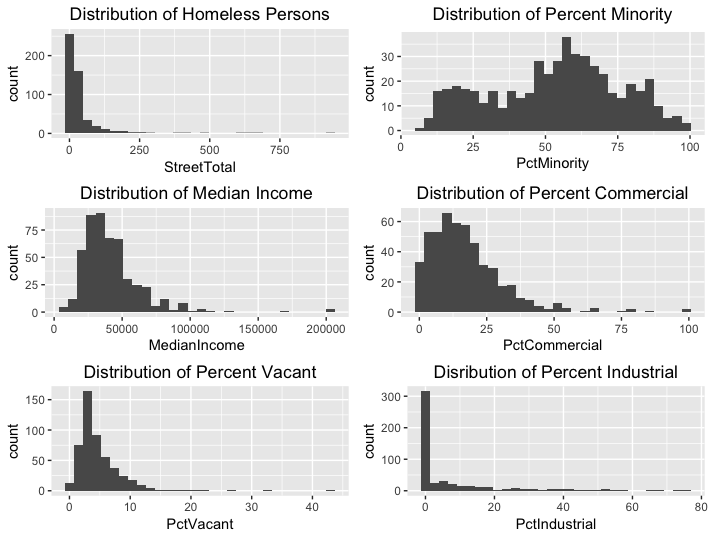
\includegraphics[scale=.65]{Histograms}
\caption{Univariate Distributions (Full Dataset)}
\end{figure}

\begin{figure} [h]
\centering
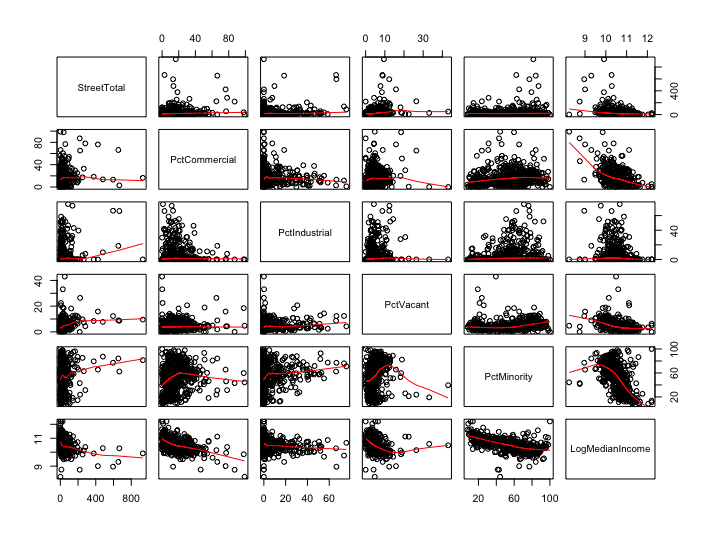
\includegraphics[scale=.65]{ScatterMatrix}
\caption{Bivariate Scatter Plot Matrix (Full Dataset)}
\end{figure}

\begin{figure} [h]
\centering
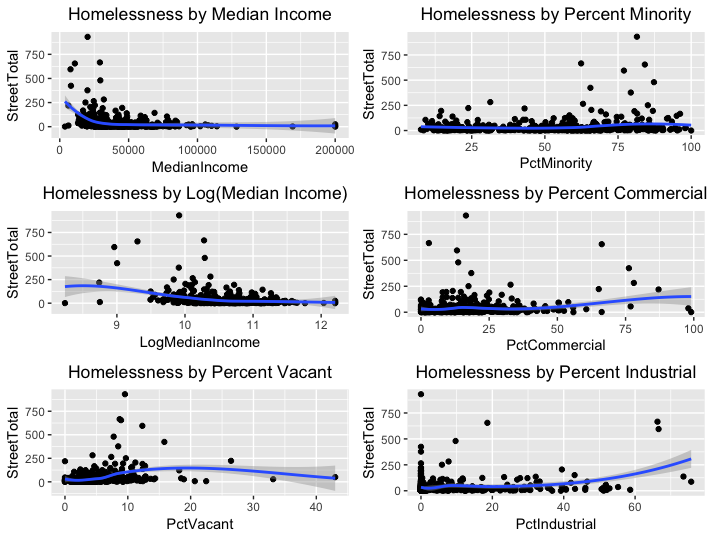
\includegraphics[scale=.65]{Scatterplots}
\caption{Bivariate Scatterplots (Full Dataset)}
\end{figure}

% Please add the following required packages to your document preamble:
% \usepackage{booktabs}
\begin{table}[]
\centering
\caption{Optimal Values of Tuning (Smoothing) Parameters}
\label{my-label}
\begin{tabular}{@{}lll@{}}
\\[-1.8ex]\hline 
\hline \\[-1.8ex] 
Percent Vacant & Percent Commercial & Percent Industrial \\ \hline
0.01068149     & 0.0007017911       & 0.005727646       \\  \hline
\multicolumn{2}{p{.5\textwidth}}{Note. Parameters are a factor of 20.}
\end{tabular}
\end{table}

\begin{sidewaystable}[]
\centering
\caption{Generalized Additive Model Results}
\label{my-label}
\begin{tabular}{llllll}
\\[-1.8ex]\hline 
\hline \\[-1.8ex] 
Parametric Coefficients: &  &  &  &  &  \\ \hline
 & Estimate & Std. Error & t-value & P-value & Significance \\  \hline 
(Constant) & 229.50408 & 136.51673 & 1.681 & 0.0949 & ns \\
Log of Income & -17.94125 & 12.34217 & -1.454 & 0.1482 & ns \\
Percent Minority & -0.04182 & 0.22082 & -0.189 & 0.8500 & ns \\

\\[-1.8ex]\hline 
\hline \\[-1.8ex] 
Approx. significance of smooth terms: &  &  &  &  &  \\ \hline
 & Edf & Ref.df & F & P-Value & Significance \\ \hline
Percent Vacant & 6.084 & 7.214 & 2.574 & 0.01436 & * \\
Percent Commercial & 8.417 & 8.896 & 3.066 & 0.00224 & ** \\
Percent Industrial & 6.373 & 7.523 & 8.373 & 0.0000 & *** \\
\\[-1.8ex]\hline 
\hline \\[-1.8ex] 
R-sq.(adj)= 0.483 &  & Deviance Explained = 55.3\% &  &  &  \\
GCV= 3094.7 &  & Scale est. = 2657.6 &  & N= 169 &  \\ \hline
p\textless.001 *** , p\textless.01 ** , p\textless.05 * &  &  &  &  &  \\ \hline
\multicolumn{2}{p{.5\textwidth}}{Note. Results computed from test data after tuning training and evaluation data with smoothing parameters.}
\end{tabular}
\end{sidewaystable}

\begin{figure} [h]
\centering
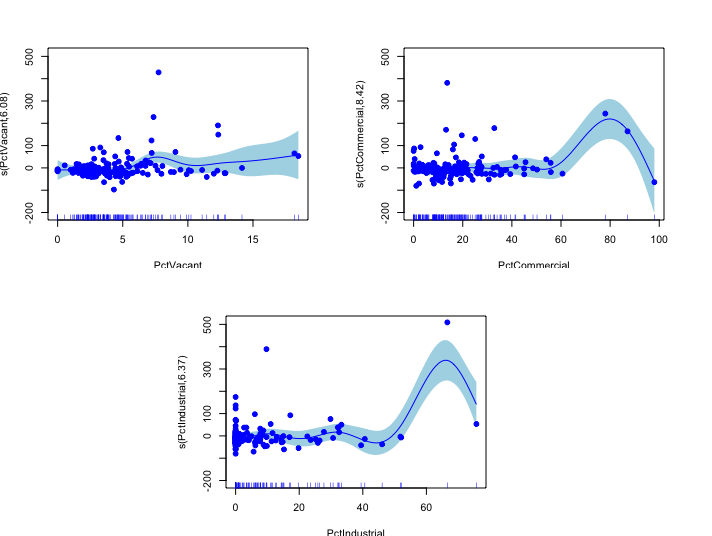
\includegraphics[scale=.65]{GAM_ALL}
\caption{Correlates of the Number of Homeless Persons per Census Tract, Los Angeles County}
\floatfoot{Rug plots with error bands are shown, n = 169}
\end{figure}






\end{document}  